%----------------------------------------------------------------------------
\chapter{Implementation}
%----------------------------------------------------------------------------

In order to validate our approach, an implementation was created. Of the subsequent sections, Section \ref{sec_tooling} discusses the utilized tools, and Section \ref{sec_interactivelearningframework} elaborates on the steps taken to provide a proof of concept implementation of the proposed \textit{Interactive Learning Entity} as an \textit{Interactive Learning Framework}.
%----------------------------------------------------------------------------
\section{Tooling} \label{sec_tooling}
%----------------------------------------------------------------------------
%TODO: random bevezeto szoveg

%----------------------------------------------------------------------------
\subsection{Eclipse Environment} \label{subsec_emf}
%----------------------------------------------------------------------------
Eclipse is a popular, open-source integrated development environment (IDE). It is mainly used for Java-related application development, but also supports several other programming languages. It consists of a base workspace and an extensible plug-in system. Using this plug-in system, the develpment environment is easily customizable for different purposes, such as programming in different programming lanugages, modeling (using the Gamma Framework or Yakindu), or testing.

\textbf{Eclipse Modeling Framework}

The Eclipse Modeling Framework is an Eclipse-based modeling framework and code generation facility. It defines its own structured data model -- called Ecore -- for describing models and providing runtime support for the models. Models are defined using the XML Metadata Interchange (XMI) format, which is supported by various Eclipse plugins developed specifically for this purpose, as EMF is fully integrated into the Eclipse platform. It provides an environment to numerous technologies, including server solutions, persistence frameworks, UI and transformation frameworks.

%----------------------------------------------------------------------------
\subsection{Xtext Framework} \label{subsec_xtext}
%----------------------------------------------------------------------------
Xtext is an open-source framework for developing (mostly) domain-specific languages (DSLs). It has its own syntax for the definition of textual languages, resembling a context-free grammar extended with mappings to the in-memory representations. Unlike standard parser generators, it generates not only a parser, but also the abstract syntax tree (AST) of the grammar, and also support several other features, such as validation rules and editing support. This is because Xtext is based on the EMF project -- the metamodels of the defined languages are Ecore models --, and it is integrated into the Eclipse environment.

\textbf{Xtend}

Xtend is a general-purpose, high-level programming language based on Java. It is statically typed, object-oriented and uses the type system of Java. Xtend programs are compiled to Java code, thus allowing seamless integration with existing Java libraries. It provides numerous convenient extensions to Java, such as dispatch methods, type inference, operator overloading and extension methods.

%----------------------------------------------------------------------------
\subsection{Sirius} \label{subsec_sirius}
%----------------------------------------------------------------------------
Sirius is an open-source project for developing graphical modeling languages. It is integrated into the Eclipse environment, enabing the specification of viewpoints for EMF models, thus the creation of graphical views. In a Sirius workbench (editor), the elements of the viewpoint specification models are mapped to individual EMF model elements, thus allowing their graphical interpretation and editing. The whole viewpoint definition procedure is declarative, using OCL \cite{OCLStandard} (or Acceleo Query Language, AQL) expressions for the traversal of the diagram elements when needed.

Sirius supports various representation types. Traditional Sirius diagrams consist mainly of nodes and edges between nodes, suitable for models in which the position of the diagram elements carries no meaning - like several structural modeling languages. It also supports table and tree representations, and also \textit{sequence diagrams} for modeling behavior - in which the position on the diagram is also part of the semantics.

%----------------------------------------------------------------------------
\subsection{Owl} \label{subsec_owl}
%----------------------------------------------------------------------------

Owl \cite{Owl} is a tool collection for $\omega$-words, $\omega$-automata and linear temporal logic. It provides several algorithms for automata and LTL, supporting - among others - LTL expression parsing and simplification, reading and writing $\omega$-automata using the HOA format \cite{HOAFormat}, translation of LTL formula to $\omega$-automata with several possible acceptance conditions, and operations over $\omega$-automata, such as product, SCC decomposition emptiness checks and acceptance-condition transformations.

Through providing these algorithms, the library supports easy development and fast prototyping in the area of LTL and automata, thus also enabling rapid concept validation.

%----------------------------------------------------------------------------
\subsection{Automata Learning Framework} \label{subsec_automatonlearning}
%----------------------------------------------------------------------------
In order to give a foundation to the implementation described in this thesis, a previously created automata learning framework TODO: ref BSC] was extended upon. Since the framework was implemented using the Java programming language, the high-level view seen in Figure \ref{fig_automatalearning_packages} is represented as an UML class diagram of the packages and the relations between them, essentially being an overview of the modularization of the framework. 


\smallskip

The \textit{Learnable} package contains the input formalisms, and the \textit{Hypothesis} package contains the output formalisms. Both are used by the teacher (\textit{Teacher} package) and the learner (\textit{Algorithm} package). The \textit{Adapter} package is used as an abstraction layer to separate the algorithm and the teacher from the input formalism. Since automaton learning algorithms have no direct access to the system under learning, and generally operate in a black-box way, the adapter package provides flexibility on what inputs can be used. As Figure \ref{fig_automatalearning_packages} illustrates, no such adapter is used on the output layer, since Hypotheses are directly accessed by the learning algorithms, and are constructed during the learning. The relations between the packages (modules) are straightforward.  Composition is used, to indicate, that there is no \textit{Algorithm} (learner) without a \textit{Teacher}, there is no \textit{Teacher} without an \textit{Adapter}, and there is no \textit{Adapter} without an input, a \textit{Learnable}, to adapt. \\
The advantage of such architecture is that the automaton learning algorithms implemented within can be agnostic to the formalism of the input provided. This results in high re-usability of the core algorithms, while being easily extensible and adaptable to arbitrary systems to infer.  

\begin{figure}[!ht] 
	\centering
	%\fbox{
	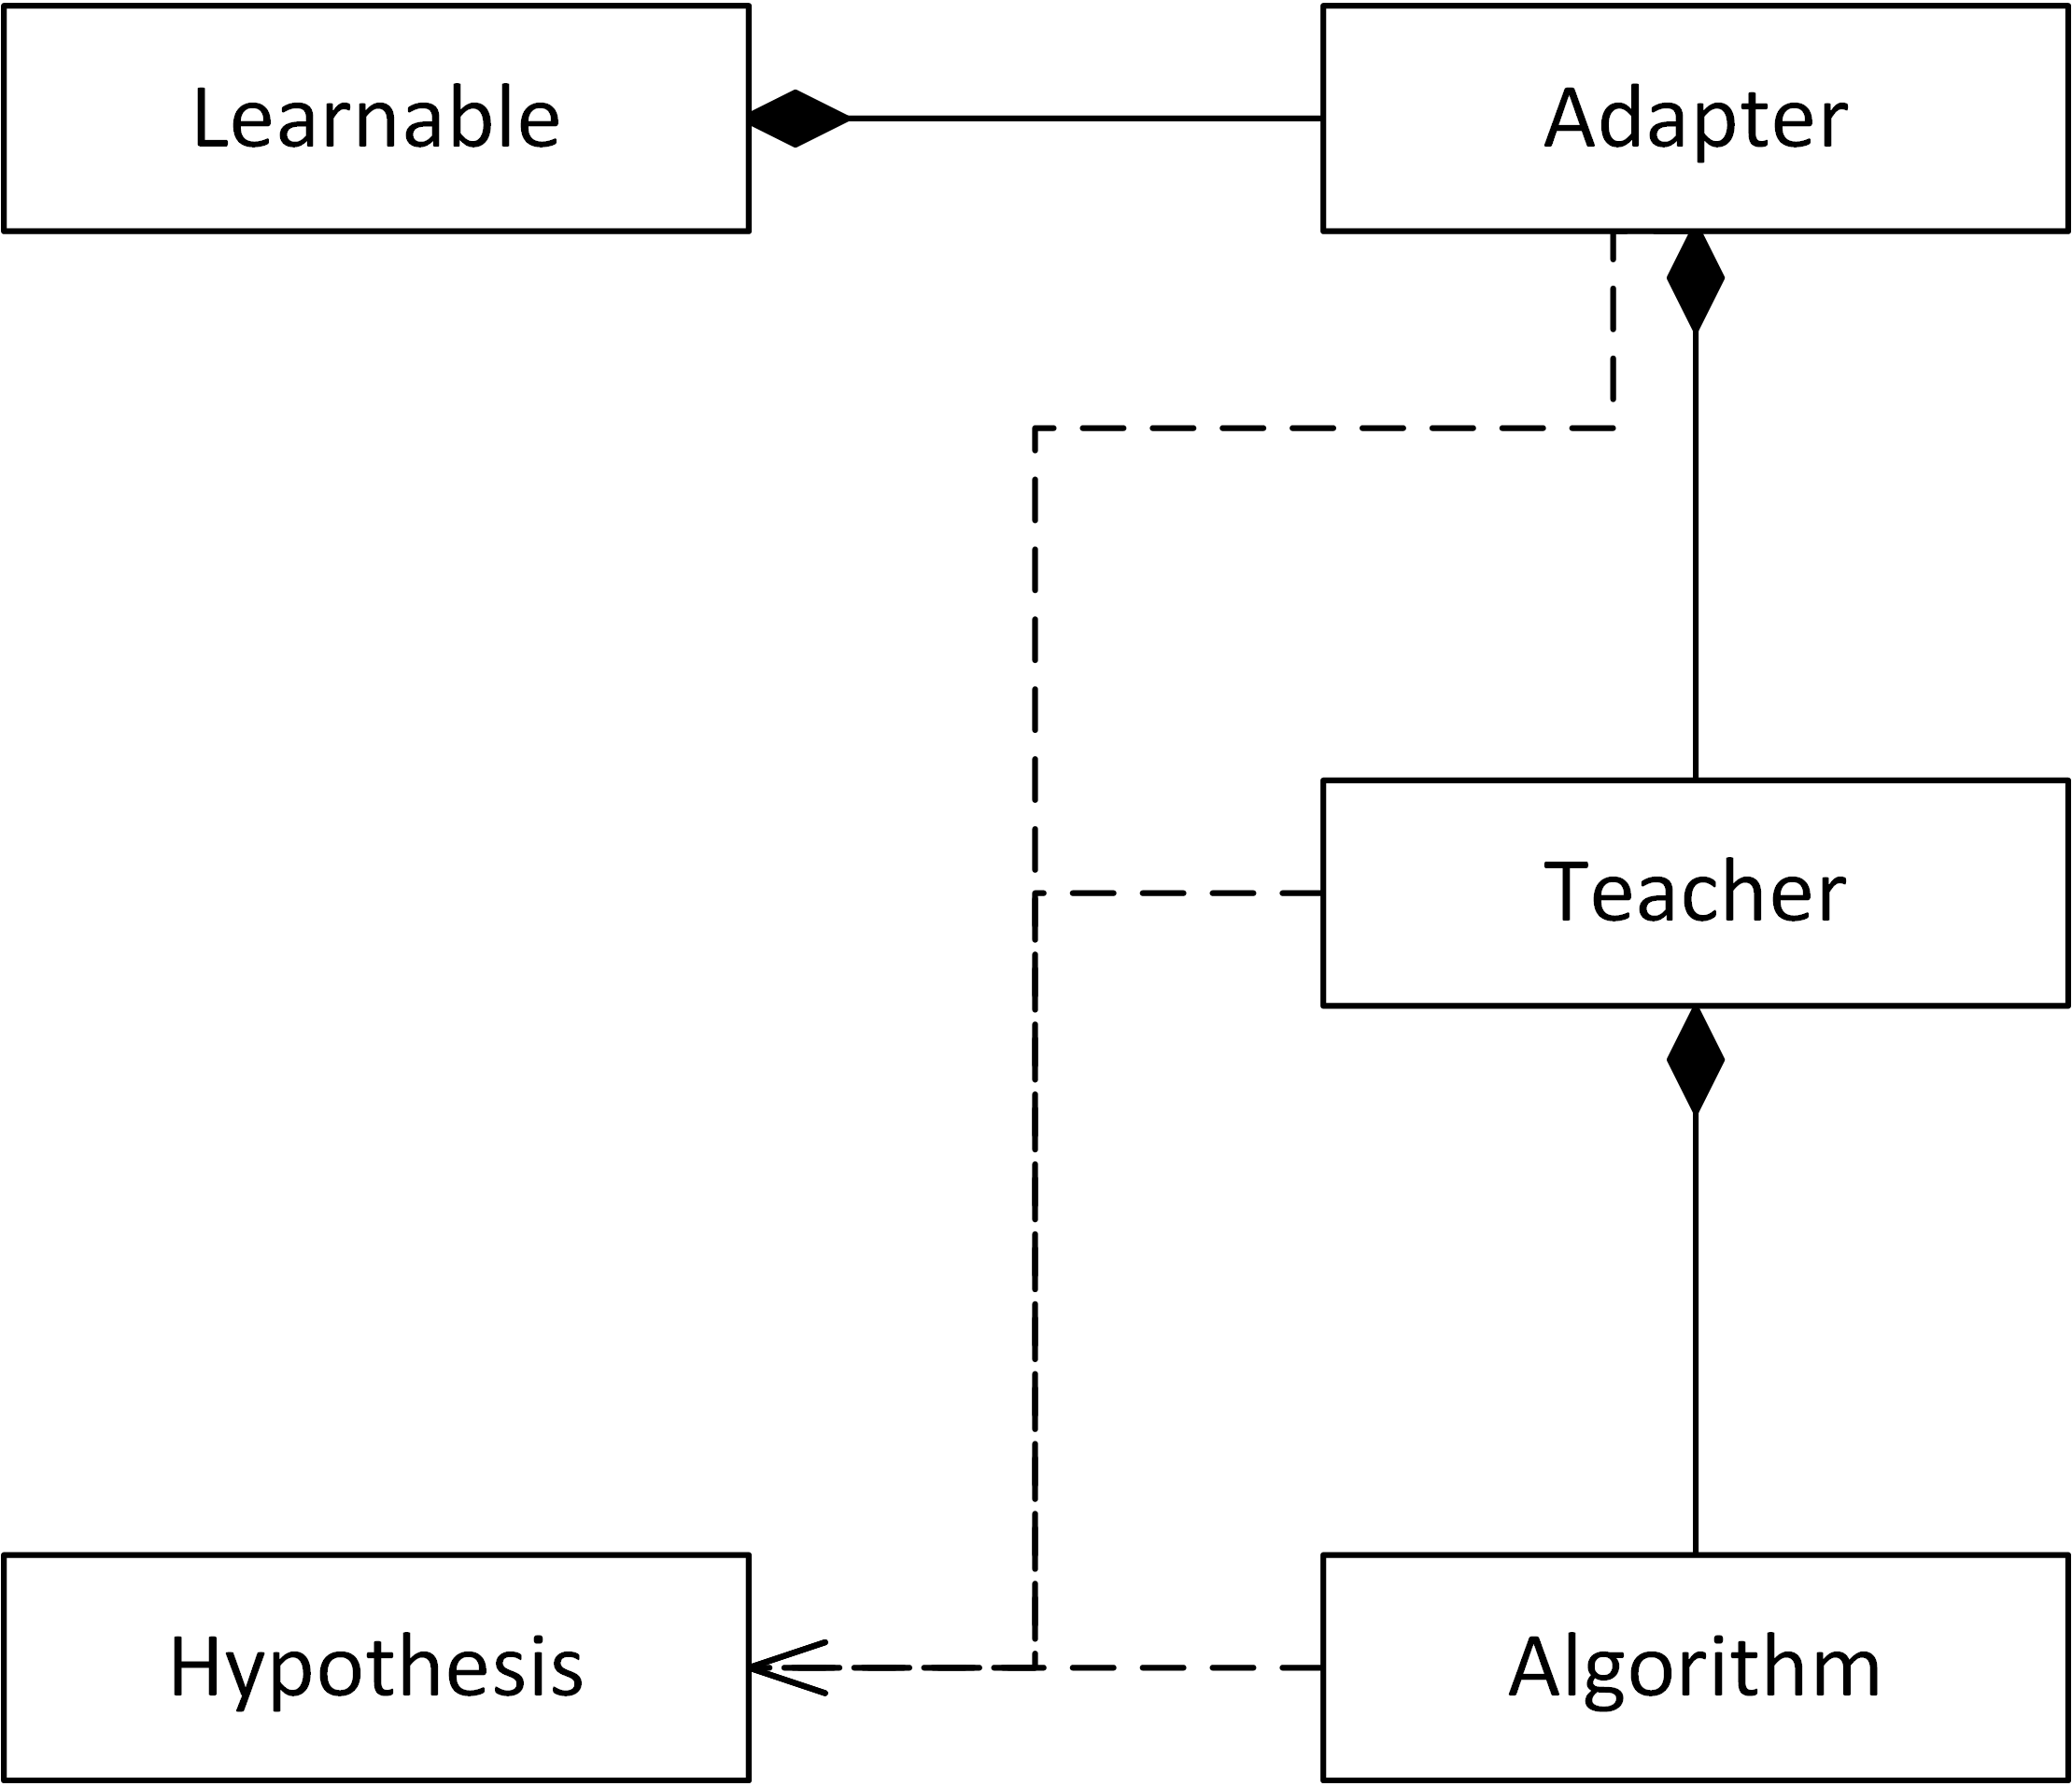
\includegraphics[width=75mm, keepaspectratio]{figures/automatalearning_packages.png}
	%}
	\caption{Structure and relations of the packages comprising the Automata Learning Framework TODO:REF BSC} 
	\label{fig_automatalearning_packages}
\end{figure}

\smallskip

%----------------------------------------------------------------------------
\section{Interactive Learning Framework} \label{sec_interactivelearningframework}
%----------------------------------------------------------------------------
%TODO: random bevezeto szoveg + fig 4.1 kiterjesztett változata - szagatott részekkel keretezve pl az Oracle



\begin{figure}[!ht] 
	\centering
	%\fbox{
	\includegraphics[width=75mm, keepaspectratio]{figures/automatonlearning_overview.png}
	%}
	\caption{Structure and relations of the packages comprising the Automata Learning Framework TODO:REF BSC} 
	\label{fig_automatonlearning_overview}
\end{figure}

%----------------------------------------------------------------------------
\subsection{The Oracle} \label{subsec_oracleimpl}
%----------------------------------------------------------------------------
The \textbf{interactive learnable} is the main part of the oracle component, responsible for storing models created from the provided reqirements and answering questions of the learning algorithm. In case of adaptive learning algorithms, it also provides information about its ability to automatically explore the design space, thus enabling the optimization of the number of questions the user has to answer. The current implementation provides three commands: \textit{optimistic}, \textit{pessimistic} and \textit{reset}.

The optimistic command represents the partial models containing more information around the given input sequence. This means, that a longer input sequence with the current one as its prefix could be answered too. 

The pessimistic command represents the partial modens not containing information around the given input sequence. Pessimistic commands are given when the optimistic command is not appropriate.

The reset command represents partial model inconsistency. This is necessary, as the user may freely add and remove requirements -- thus models -- which may be contradicting each other. In case such an inconsistency is detected, the user removes a model, which may remove previously collected information. Thus, the learning must be restarted with the remaining models. Other components -- like the cache -- are also affected by the reset command.

The \textbf{LTL parser} is a simple parser implemented using the Xtext framework. It creates a DOM from the LTL expression provided by the user based on the corresponding Ecore metamodel, which then can be used by the other components. It is responsible for the introduction of the event semantics into the provided expressions, as described in Subsection \ref{subs_reqtypes}. It is also able to serialize the expressions to different formats.

%----------------------------------------------------------------------------
\subsection{The Learning Algorithm} \label{subsec_adaptivedhc}
%----------------------------------------------------------------------------
%TODO: DHC, adaptive teacher

%----------------------------------------------------------------------------
\subsection{Caching} \label{subsec_memoization}
%----------------------------------------------------------------------------
%TODO: memoizinglearnable

